%% Overleaf			
%% Software Manual and Technical Document Template	
%% 									
%% This provides an example of a software manual created in Overleaf.

\documentclass{ol-softwaremanual}



%tikz packages
\usepackage{tikz}
\usepackage{adjustbox}
\usetikzlibrary{arrows.meta,
                chains, automata,
                positioning,
                shapes.geometric,
                %bayesnet,
                backgrounds,
                decorations.pathreplacing
                }

\newcommand{\edgex}[3][style={-latex}]{% edge with a new style <<<
	% Connect all nodes #2 to all nodes #3.
	\foreach \x in {#2} { %
		\foreach \y in {#3} { %
			\draw[#1,->] (\x) -- (\y) ;%
		} ;
	} ;
}
\tikzset{
  main/.style={circle, minimum size = 1.1cm, thick, draw =black!80, node distance = 10mm}
}

% Packages used in this example
\usepackage[colorlinks=true, urlcolor=blue, linkcolor=red]{hyperref}
\usepackage{graphicx}  % for including images
\usepackage{microtype} % for typographical enhancements
\usepackage{minted}    % for code listings
\usepackage{amsmath}
\usepackage{amsfonts}
\usepackage{amssymb}
\setminted{style=friendly,fontsize=\small}
\renewcommand{\listoflistingscaption}{List of Code Listings}
\usepackage[a4paper,top=4.2cm,bottom=4.2cm,left=3.5cm,right=3.5cm]{geometry} % for setting page size and margins
\usepackage{cleveref}

% Custom macros used in this example document
\newcommand{\doclink}[2]{\href{#1}{#2}\footnote{\url{#1}}}
\newcommand{\cs}[1]{\texttt{\textbackslash #1}}

% Frontmatter data; appears on title page
\title{Short guidance}
\version{1.0.0}

\softwarelogo{
\includegraphics[width=8cm]{ICFEP-UQLOGO.png}}
% redefine \VerbatimInput
\RecustomVerbatimCommand{\VerbatimInput}{VerbatimInput}%
{fontsize=\footnotesize,
 %
 frame=lines,  % top and bottom rule only
 framesep=2em, % separation between frame and text
 labelposition=topline,
 %
 commandchars=\|\(\), % escape character and argument delimiters for
                      % commands within the verbatim
 commentchar=*        % comment character
}





\begin{document}

\maketitle

\tableofcontents
\listoflistings
\newpage
\section{Welcome to ICFEP-UQ guidance!}\label{ICFEP-UQ_setup}
ICFEP-UQ is a general purpose and Matlab-based toolbox for modelling uncertainty in physical and mathematical systems. The application of the code can be generalized to ABAQUS/PLAXIS/etc and all kinds of engineering problems. The code is organized as a set of modules centered around core capabilities in Uncertainty Quantification (UQ).
\begin{table}[htbp]
\begin{tabular}{|l|l|}
\hline
\textbf{Product owner:} & Truong Le       \\ \hline
Lead developers:        & Ningxin Yang    \\ \hline
Contributors:           & Master students \\ \hline
\end{tabular}
\end{table}

All primary functionalities in ICFEP-UQ are categorized as:
\begin{itemize}
    \item Sequential Bayesian inference
    \item Enriching experimental design
    \item Sensitivity Analysis 
    \item Dimensionality reduction based surrogate models 
    \item User-defined loglikelihood for combined data sources (ongoing)
\end{itemize}

\subsection*{Software/system preparation}
\textbf{Dependencies required:}
\begin{verbatim}
MATLAB® R2019a and later; windows; 
Uqlab package (version 2.1); 
Statistics and Machine learning toolbox,
...
\end{verbatim}

\textbf{Installation:}\\
For MATLAB, Imperial holds license. For UQlab opensource package, you can download it from \href{https://www.uqlab.com/install}{here} and following the basic installation within.

\textbf{Contact:}\\
n.yang23@imperial.ac.uk

\section{Theory basis}
\subsection*{Probabilistic theory}
\textit{Sum rule} and \textit{product rule} are the basis of \textit{Bayes theorem}. \\
Relationship between \textit{integration} and \textit{expectation}.\\
Basis knowledge on first and second \textit{moments}.\\
...\\
See \href{https://www.britannica.com/science/probability-theory}{more details}



\subsection*{Bayesian inference}
\textit{Frequentist vs Bayesian} \\
\textit{Bayes theorem} \\
\textit{Inference} - \textit{prior}, \textit{likelihood} and \textit{evidence}\\
\textit{Sampling methods to posterior}





\subsection*{Sequential Bayesian inference}
In engineering problems, observations are acquired stage by stage based on construction/loading. Therefore, the Bayesian inference/model calibration is conducted step by step, which is also called \textit{sequential Bayesian inference}. Based on a Markovian process, some problems are \textit{filtering, smoothing and prediction}.

\begin{adjustbox}{width=7cm}
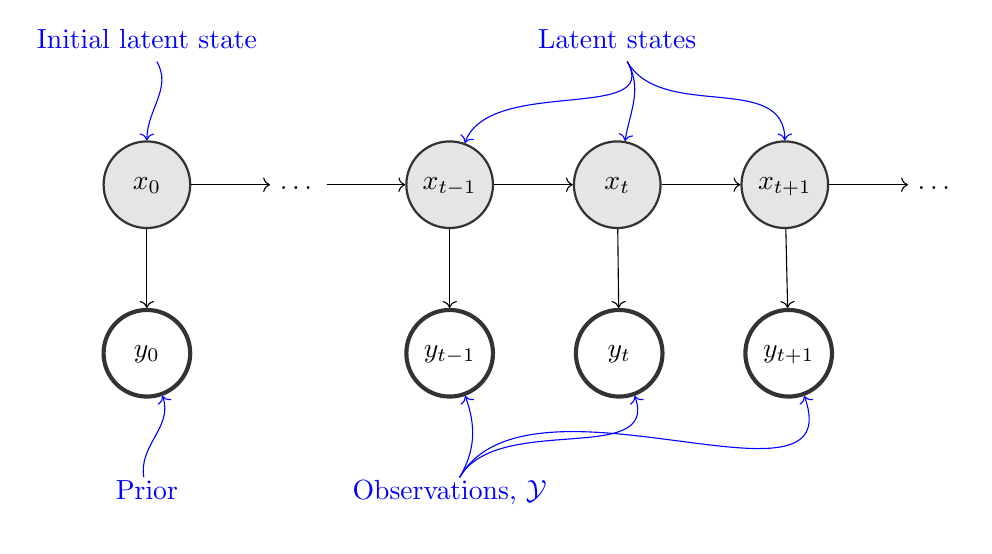
\begin{tikzpicture}[%
				x=1.0cm, y=0.6cm,
				every node/.style={
					text height=1ex,
					text depth=.25ex,
				},]
				
				% nodes
				\node[main,line width = 1.5pt] (x0) {$y_{0}$};%
				\node[main,above=of x0,fill=black!10] (y0) {$x_{0}$}; %
				\node[right=of y0] (dotsy) {$\dots$};
				\node[main, right= of dotsy,fill=black!10] (y-1) {$x_{t-1}$}; %
				\node[main, below= of y-1,line width = 1.5pt] (x-1) {$y_{t-1}$};%
				\node[main, right= of x-1,line width = 1.5pt] (x) {$y_{t}$};%
				\node[main, right= of y-1,fill=black!10] (y) {$x_{t}$}; %
				\node[main, right= of x,line width = 1.5pt] (x+1) {$y_{t+1}$};%
				\node[main, right= of y,fill=black!10] (y+1) {$x_{t+1}$}; %			
				\node[right=of y+1] (dotsy2) {$\dots$};	
				
				\node[below=of x0] (prior) {\color{blue} Prior};
				\node[below=of x-1] (obs) {\color{blue} Observations, $\mathcal{Y}$};
				\node[above=of y] (main) {\color{blue}Latent states};
				\node[above=of y0] (initial) {\color{blue} Initial latent state};

				% edges 
				\edgex {y0} {x0}; %
				\edgex {y0} {dotsy}; %
				\edgex{dotsy} {y-1} ; %
				\edgex {y-1} {x-1}; %
				\edgex {y} {x}; %
				\edgex {y-1} {y}; %				
				\edgex {y} {y+1}; %
				\edgex {y+1} {x+1}; %
				\edgex {y+1} {dotsy2}; %
				
				\draw [->,blue] (prior) to[out=+100,in=-70] (x0);
				\draw [->,blue] (obs) to[out=+60,in=-70] (x-1);
				\draw [->,blue] (obs) to[out=+60,in=-70] (x);
				\draw [->,blue] (obs) to[out=+60,in=-70] (x+1);
				
				\draw [->,blue] (main) to[out=-60,in=+70] (y-1);
				\draw [->,blue] (main) to[out=-60,in=+80] (y);			
				\draw [->,blue] (main) to[out=-60,in=+90] (y+1);					
				\draw [->,blue] (initial) to[out=-60,in=+90] (y0);				
				%label
				\end{tikzpicture}
    \end{adjustbox}
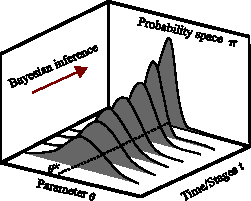
\includegraphics[scale=1]{figures/figure-SBI.pdf}








\subsection*{Components in UQ}
Four components in uncertainty quantification
\begin{itemize}
    \item Model assessment
    \item Model calibration
    \item Uncertainty propagation
    \item Sensitivity analysis
\end{itemize}
\begin{figure}[htbp]
    \centering
    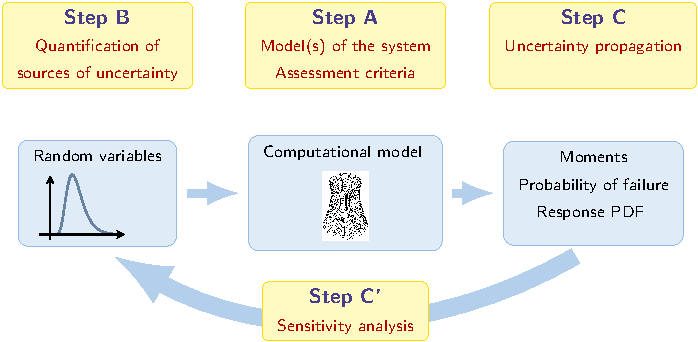
\includegraphics{figures/figure-UQ_components_bruno.pdf}
    \caption{UQ framework}
    \label{fig:UQ_framework}
\end{figure}




\section{Sensitivity analysis}
\textit{Sampling methods to input space}\\
\textit{Sobol's indice}\\
\textit{PC expansion-Sobol's indice}\\
\textit{PCA-PCE-Sobol's indice} 


\section{Uncertainty propagation}
\textit{Prior predictive} and \textit{posterior predictive} distributions are very important indicators for assessing the predictive ability of the model and uncertainties propagation in output space.

The \textit{prior predictive} distribution can be represented as:
\begin{equation}
    \label{eq: prior predictive}
    \pi({\boldsymbol{\mathsf{y}}}) = \int_{\mathcal{D}_{\boldsymbol{X}}} 
    \pi(\boldsymbol{x}) \pi({\boldsymbol{\mathsf{y}}}|\boldsymbol{x}) {\rm{d}} \boldsymbol{x}
\end{equation}
where ${\boldsymbol{\mathsf{y}}}$ is the simulator prediction, $\boldsymbol{x}$ are the input parameters. It summarises the uncertainty about the model output considering the discrepancy model before calibration. In practice, it is used to determine whether the measured data can be reproduced. It is essential for identifying and ruling out challenging inverse problems before proceeding with expensive calibration procedures. 

The \textit{posterior predictive} distribution can be similarly written as:
\begin{equation}
    \label{eq: posterior predictive}
    \pi({\boldsymbol{\mathsf{y}}}|\mathcal{Y}) = \int_{\mathcal{D}_{\boldsymbol{X}|\mathcal{Y}}} 
    \pi(\boldsymbol{x}|\mathcal{Y}) \pi({\boldsymbol{\mathsf{y}}}|\boldsymbol{x}) {\rm{d}} \boldsymbol{x}
\end{equation}
It gives model predictions for future stages based on the current inferred parameters $\boldsymbol{X}$. 


\section{Model assessment}
In the UQ setting, especially for geotechnical problems, engineers will use very complex and advanced constitutive models. Each run will cost hours to days, in this case, original simulator $\mathcal{M}$ will and must be replaced by a cheap-to-evaluate surrogate $\Tilde{\mathcal{M}}$ to accelerate the running speed.
\begin{figure}[htbp]
    \centering
    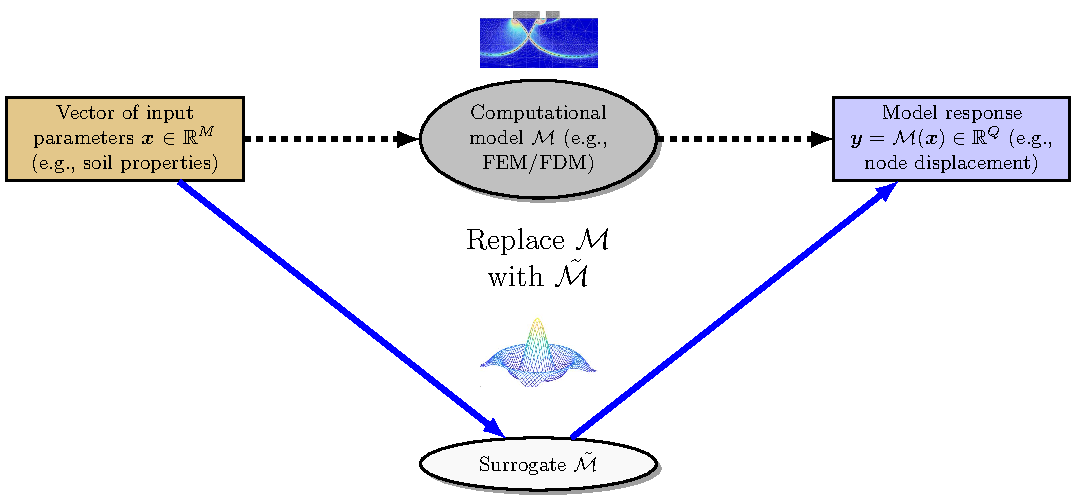
\includegraphics[width = 90mm]{figures/figure-UQ_surrogate.pdf}
    \caption{Surrogate to replace original simulator}
    \label{fig:UQ_surrogate}
\end{figure}

Currently, ICFEP-UQ are using dimensionality reduction-based surrogates. Basically, \textit{principal component analysis} is used for feature extraction and dimensionality reduction. Then a surrogate is built directly on these reduced-order spaces. And this will benefit in two ways: (1) accelerate the Bayesian inference process; (2) capture the connections among output points and give more accurate model predictions. 

Dimensionality reduction techniques are only supporting:
\begin{itemize}
    \item Principal component analysis
\end{itemize}

Some surrogates choices in ICFEP-UQ are:
\begin{itemize}
    \item Polynomial chaos expansion
    \item Polynomial chaos kriging
    \item Stochastic spectral embedding
\end{itemize}


\section{Model calibration}
\textit{Bayesian inference} or \textit{model calibration} is the most challenging part in UQ. Because it requires designers having a high-level understanding of:
\begin{itemize}
    \item Working flow of sequential Bayesian inference 
    \item Error types from observations, model discrepancy and surrogates
    \item User-defined loglikelihood function
\end{itemize}

Connecting the reality with simulator $y \leftrightarrow \mathcal{M}(\boldsymbol{x})$ as: 
\begin{equation*}
\boldsymbol{y} = \mathcal{M}(\boldsymbol{x})
+ \boldsymbol{\varepsilon}
\end{equation*}
in which, $\boldsymbol{y}$ is the observation, $\mathcal{M}(\boldsymbol{x})$ is the model prediction and $\boldsymbol{\varepsilon}$ is the error term.

Normally, it is assumed that $\boldsymbol{\varepsilon}$ is following a zero-mean Gaussian distribution because of its simple and popular form $\boldsymbol{\varepsilon} \in \mathcal{N}(\boldsymbol{\varepsilon}|\boldsymbol{0},\boldsymbol{\Sigma})$. The covariance matrix $\boldsymbol{\Sigma}$ with $N$ outputs points can be simple as an identical matrix like:
\begin{equation}
\label{eq: iid_general_discrepancy}
\boldsymbol{\Sigma} = \sigma^2 \boldsymbol{I}=
\sigma^2
  \begin{bmatrix}
1 & 0 & \hdots & 0 \\
0 & 1 & \hdots & 0 \\
\vdots & \vdots & \ddots & \vdots \\
0 & 0 & \hdots & 1 
\end{bmatrix}   
\end{equation}
or holding a more general form:
\begin{equation}
\label{eq: general_discrepancy}
\boldsymbol{\Sigma} = 
  \begin{bmatrix}
\sigma_{11} & \sigma_{12} & \hdots      & \sigma_{1N} \\
\sigma_{12} & \sigma_{22} & \hdots      & \sigma_{2N} \\
\vdots      & \vdots      & \ddots      & \vdots \\
\sigma_{N1} & \sigma_{N2} & \hdots      & \sigma_{NN}
\end{bmatrix}    
\end{equation}
The discrepancy $\boldsymbol{\varepsilon}$ follows a Gaussian distribution with unknown residuals variance $\boldsymbol{\Sigma}$. Likelihood function $\mathcal{L}$ can be expressed as:
\begin{equation}        
        \label{eq: Likelihood function}
\begin{aligned}
 \mathcal{L}(\boldsymbol{x}|\mathcal{Y}) =& N(\boldsymbol{y}|\mathcal{M}(\boldsymbol{x}),\boldsymbol{\Sigma}) \\
 =&  \frac{1}{\sqrt{(2 \pi){\rm{det}} 
 (\boldsymbol{\Sigma})}}\exp\left(-\frac{1}{2}\left(\boldsymbol{y}  - \mathcal{M}(\boldsymbol{x})\right)^{\mathsf{T}} \boldsymbol{\Sigma}^{-1}\left(\boldsymbol{y}  - \mathcal{M}(\boldsymbol{x})\right)\right)
\end{aligned}
\end{equation}
Note: $\boldsymbol{y}$ is an observation vector, which is different from FE prediction $\boldsymbol{\mathsf{y}} = \mathcal{M}(\boldsymbol{x})$.

In \Cref{eq: iid_general_discrepancy}, $\boldsymbol{\varepsilon}$ is non-informative, thus, its prior for the variance $\sigma$ follows uniform distribution $\sigma\sim \mathcal{U}$(0,$\sigma_{0}^2$), in which $\sigma_{0}^2$ should be related to the observation values (e.g., mean or maximum). $\boldsymbol{\varepsilon}$ now can be considered as some additional priors $\boldsymbol{x^{\varepsilon}}$ along with forward parameters $\boldsymbol{x}^{\mathcal{M}}$ shown as \Cref{fig:figure-Sequential_Bayesian_updating}. UQlab default setting only supports \textit{iid} assumption as shown \Cref{eq: iid_general_discrepancy}, which is very unrealistic for most engineering problems. 
 \begin{figure}[htbp]
    \centering
    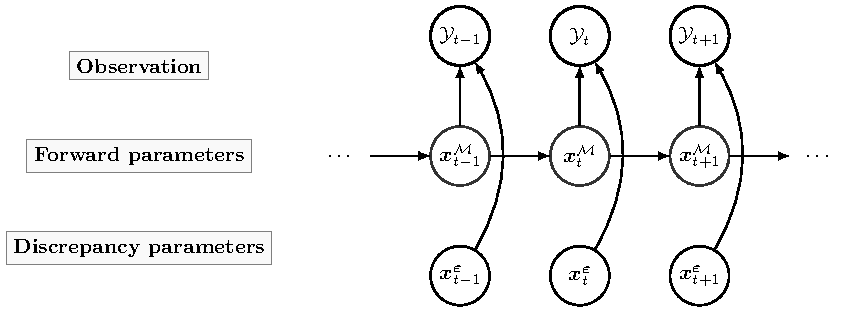
\includegraphics[width = 90mm]{figures/figure-Sequential_Bayesian_updating.pdf}
    \caption{Sequential parameter updating}
    \label{fig:figure-Sequential_Bayesian_updating}
\end{figure}
Because \textit{iid} assumption will lose all connections inside the discrepancy term. \textit{Kernel methods} are good ways to capture the connections within the covariance matrix $\boldsymbol{\Sigma}$ in $\boldsymbol{x^{\varepsilon}}$, such as:
 \begin{figure}[htbp]
    \centering
    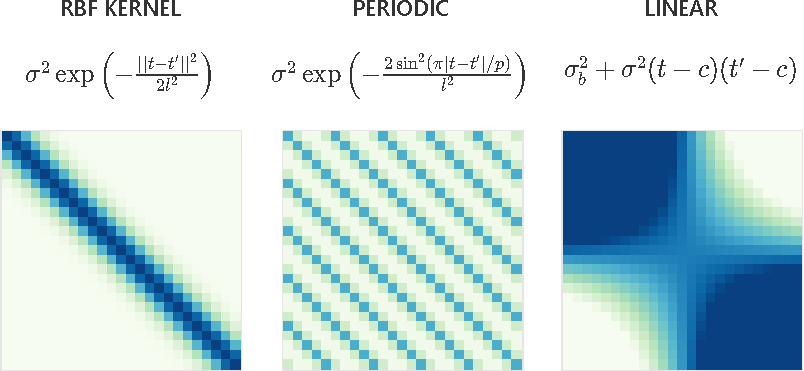
\includegraphics[width = 90mm]{figures/figure-kernel.pdf}
    \caption{Some kernel choices}
    \label{fig:figure-kernel}
\end{figure}

\textbf{Things are not done yet}. Even we know the the connection of discrepancy $\boldsymbol{x^{\varepsilon}}$ can be reproduced by \textit{kernel methods}. But we still need to give values for initial prior distributions to $\boldsymbol{x^{\varepsilon}}$. \textit{Kernel methods} can only reproduce the connections within the $\boldsymbol{x^{\varepsilon}}$ rather than the absolute magnitude. This is a tricky part, because $\boldsymbol{x^{\varepsilon}}$ discrepancy is actually coming from the instrument accuracy, which we dont know. If we assign a very small value, it means there is smaller error and high confidence in the observation data we obtained. On the contrary, if we give a big value, we have less confidence in the data source. Obviously, the discrepancy term $\boldsymbol{x^{\varepsilon}}$ will influence the calibration process.

\section{Example to get started}
\subsection*{Problem statement}
The problem involved the 3D simulation of laterally loaded piles in overconsolidated glacial clay till at the Cowden test site. All numerical analyses were conducted using the ICFEP, a deterministic forward simulator. The model's accuracy was verified, with the soil strength profile $s_{\text{u}}$ and staged pile outputs $\boldsymbol{y}$ as illustrated in \Cref{fig: cowdensite}. The FE pile model employed in this study conforms to the CL2 type outlined, featuring a diameter of 2.0 meters and a length ratio of $L/D = 5.25$. Given the symmetrical nature of the model, only half of the pile is modelled.
 \begin{figure}[htbp]
    \centering
    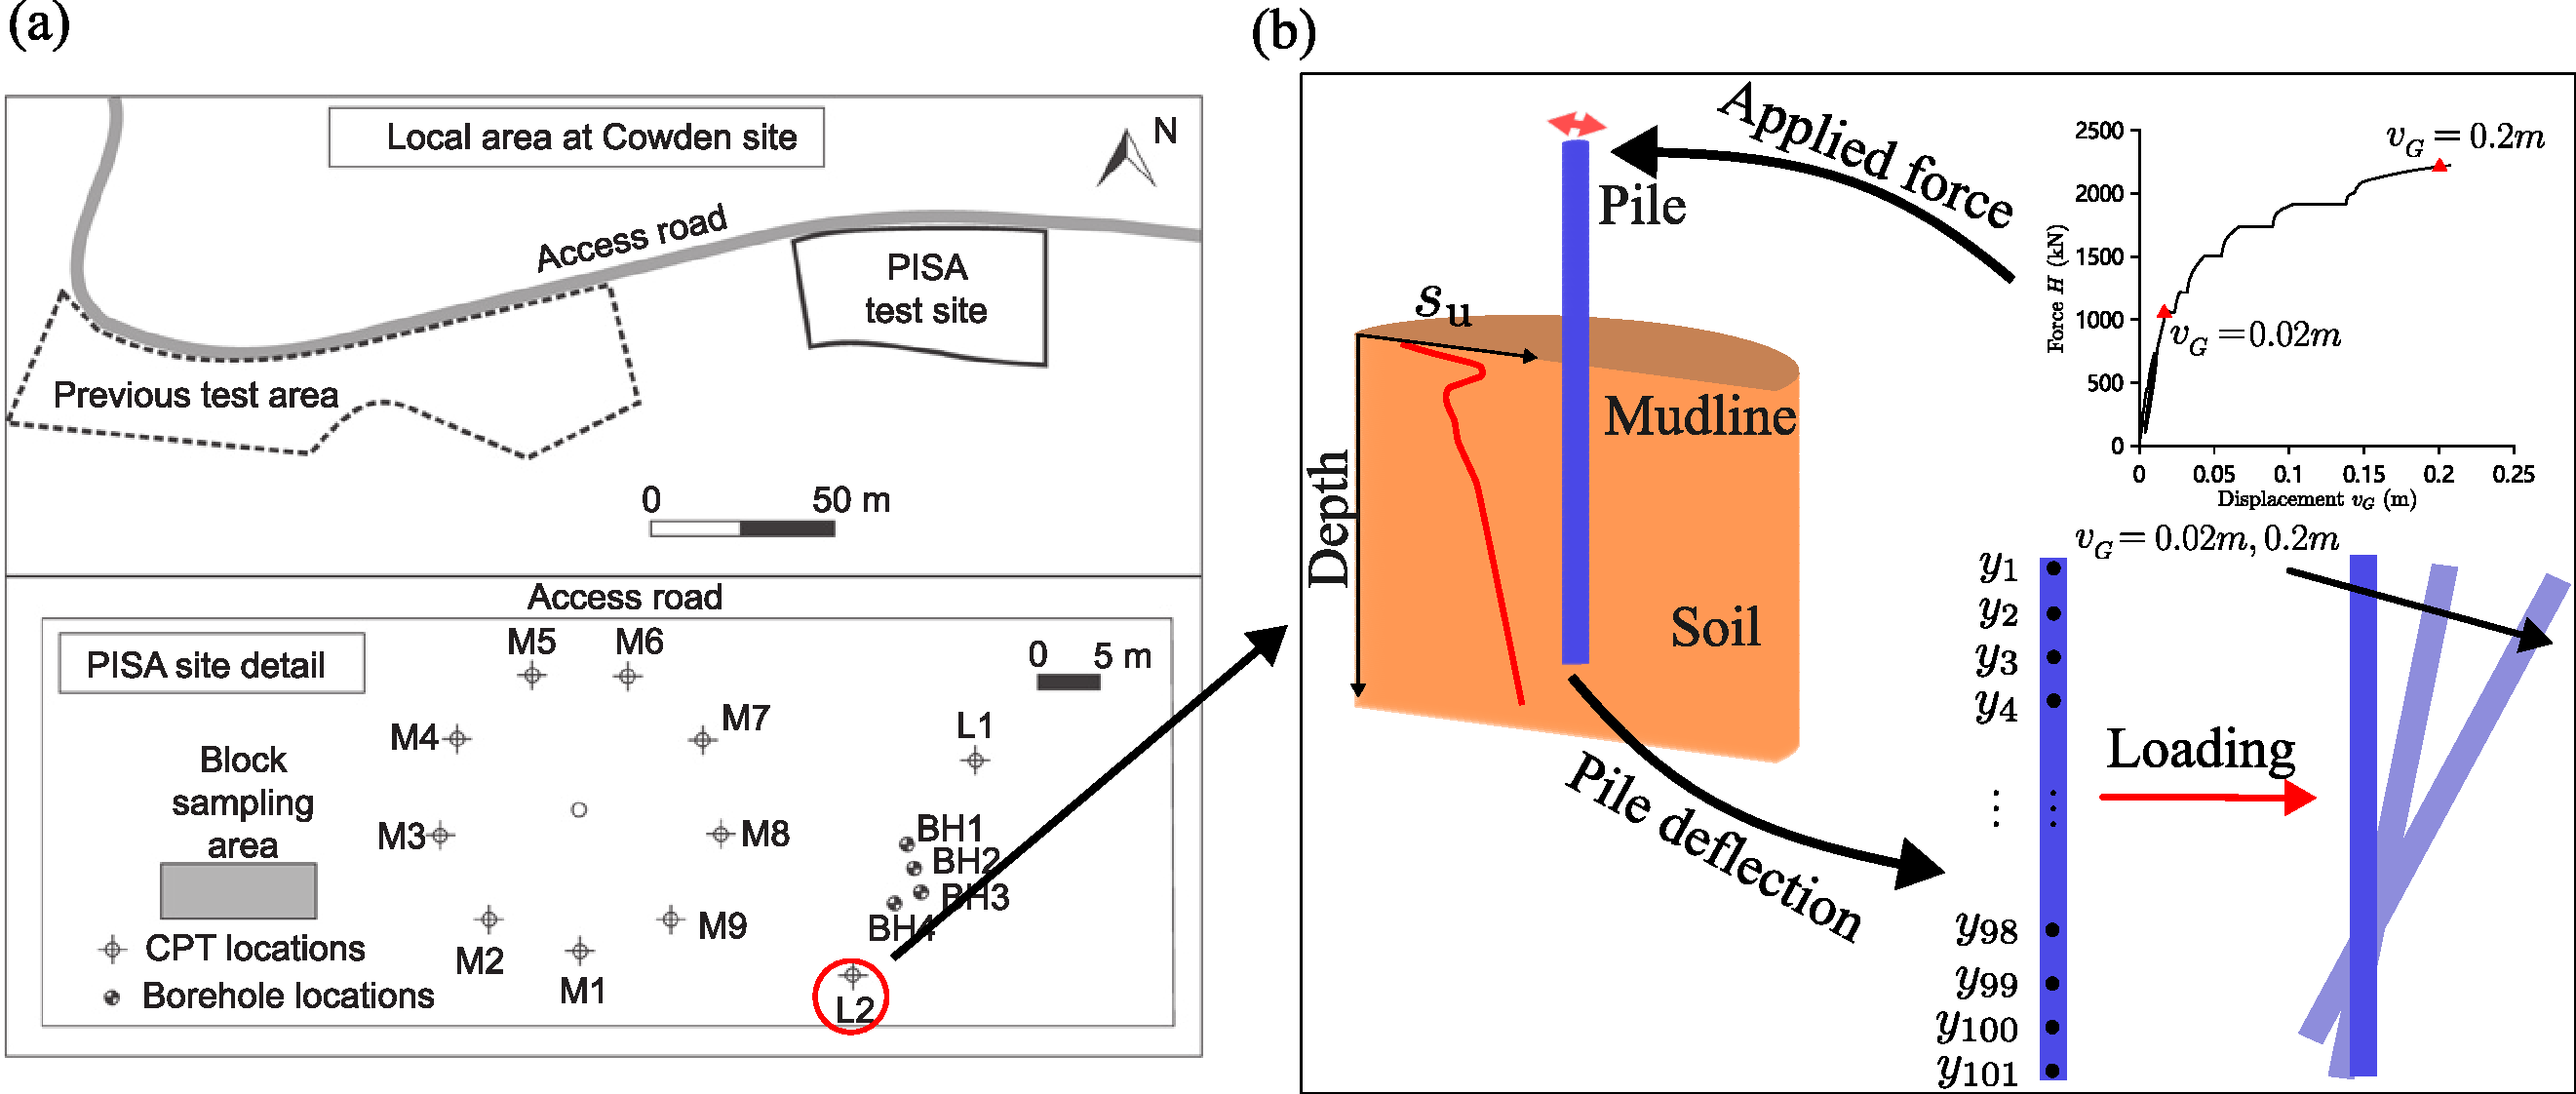
\includegraphics[width = 140mm]{figures/figure-cowden.pdf}
    \caption{Loading pile at Cowden site}
    \label{fig: cowdensite}
\end{figure}

Similar to the original investigation, laboratory data was interpreted to constructed the prior set of best-estimate parameters. This study however considers a number of parameter of the forward model as a random variables sampled from the input domain $\mathcal{D}_{\boldsymbol{x}^\mathcal{M}}$ through a distribution defined by the prior $\pi(\boldsymbol{x})$. Monotonic lateral loading was imposed at the pile head as shown in \Cref{fig: cowdensite}. Two separate measurements of deflection along the length of the pile were collected: (1) pile deflection and (2) reaction force near mudline.
\begin{itemize}
    \item Two sets of output fields: deflection and force
    \item Three parameters to be validated: $K_0$, $G_0$ and $OCR$
    \item Nine loading stages in real life/70 loading stages in FE modelling
    \item deflection output is a vector and force output is a scalar
\end{itemize}

\subsection*{Data preparation}
If this is a synthetic problem, a 'GroundTruth.csv' should be provided:
\begin{verbatim}
    ...\RUN\input\csv\ICFEP\Pisa_pile\GroundTruth.csv
\end{verbatim}
Two output fields observations : (1) pile deflection and (2) reaction force and their coordination
\begin{verbatim}
    ...\RUN\input\csv\ICFEP\Pisa_pile\Observation1.csv
    ...\RUN\input\csv\ICFEP\Pisa_pile\Observation2.csv
\end{verbatim}
Priors for forward parameters: $K_0$, $G_0$ and $OCR$
\begin{verbatim}
    ...\RUN\input\csv\ICFEP\Pisa_pile\Prior_forward.csv
\end{verbatim}
Priors for discrepancy hyperparameters: $w$ and $h$
\begin{verbatim}
    ...\RUN\input\csv\ICFEP\Pisa_pile\hyper_obs_discrepancy1.csv
    ...\RUN\input\csv\ICFEP\Pisa_pile\hyper_obs_discrepancy2.csv
\end{verbatim}
Experimental design range: for surrogate construction
\begin{verbatim}
    ...\RUN\input\csv\ICFEP\Pisa_pile\Prior_EoD.csv
\end{verbatim}
Loading stage time: FE stage time/observation time (try to make these at same coordination)
\begin{verbatim}
    ...\RUN\input\csv\ICFEP\Pisa_pile\StageTime.csv
    ...\RUN\output\mat\EoD_FE_summary\xxx.mat\FE_stagetime
\end{verbatim}
FE model evaluation: LHS input/output experimental design realization and its coordination
\begin{verbatim}
    ...\RUN\output\mat\EoD_FE_summary\xxx.mat\FEcell_output
    ...\RUN\output\mat\EoD_FE_summary\xxx.mat\EDarray
    ...\RUN\output\mat\EoD_FE_summary\xxx.mat\coord 
\end{verbatim}


\subsection*{Code setting}
Working path must be in 'xxx/Run' file
\begin{verbatim}
    ...\SBI\RUN
\end{verbatim}
Add subroutine path and UQlab core path
\begin{verbatim}
    addpath("...\UQlab\UQLab_Rel2.1.0\UQLab_Rel2.1.0\core");%UQLAB core 
    addpath("...\SBI\Main\subroutines");                    %subroutine 
\end{verbatim}
Add noise to the observation data
\begin{verbatim}
    Noise.scalar = 0;% Value as a percentage (e.g. 0.01-1.0)
\end{verbatim}
Input the FE loading stages number
\begin{verbatim}
    AnParam.N_FE_stage = 70; %number of FE loading stages
\end{verbatim}
Switches to control whether save/show the predictive distributions for the output
\begin{verbatim}
    AnParam.Switch_Predictive  =  "off";
    % switch for prior/posterior predictive for real outputs
\end{verbatim}
Validation runs setting: Keep some runs for validation
\begin{verbatim}
    AnParam.TestDataRun = 10; %Test FE runs number
\end{verbatim}
Switches to surrogate plotting figures to see the fitting degree
\begin{verbatim}
    AnParam.Switch_surrogatePlot  =  "on"; 
\end{verbatim}
Switches to corner figure plotting
\begin{verbatim}
    AnParam.Switch_corner_scatter  =  "on";
\end{verbatim}
Switches to Sobol figure plotting
\begin{verbatim}
    AnParam.Switch_Sobol  =  "on";
\end{verbatim}
Switches to threeSigma figure plotting
\begin{verbatim}
    AnParam.Switch_threeSigma  =  "on";
\end{verbatim}
Switches to show figures in matlab live script or save outside the matlab
\begin{verbatim}
    AnParam.figureDisplay =  "Show-in-mlx";
\end{verbatim}
All other switches not mentioned dont suggest using


\subsection*{Code running}


\end{document}
